\documentclass{standalone}
\usepackage[T1]{fontenc}
\usepackage[latin2]{inputenc}
\usepackage[english]{babel}
\usepackage{tikz}
\usepackage{times}
\usetikzlibrary{calc,through,backgrounds,positioning,fit}
\usetikzlibrary{shapes,arrows,shadows}
 
\begin{document}
 
\tikzstyle{place}=[shape=circle, draw, minimum height=10mm]
\tikzstyle{trig}=[shape=circle, draw, dashed, minimum height=10mm]
\tikzstyle{trans}=[shape=rectangle, draw, minimum height=6mm, minimum width=12mm]
 
\centering
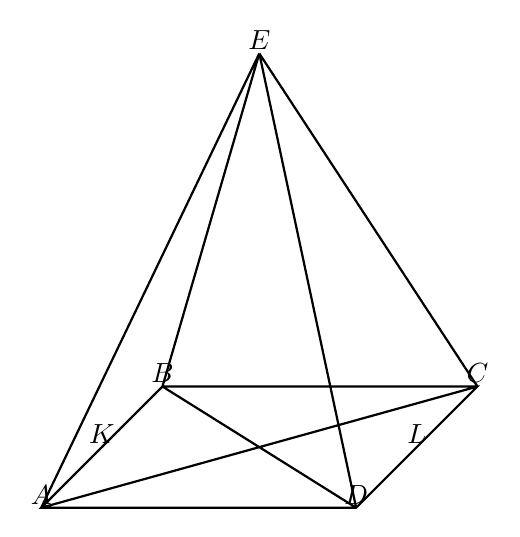
\begin{tikzpicture}[scale=1,inner sep=0.4mm]
\coordinate[label = {$A$}] (A) at (0,0,4);
\coordinate[label = {$B$}] (B) at (0,0,0);
\coordinate[label = {$C$}] (C) at (4,0,0);
\coordinate[label = {$D$}] (D) at (4,0,4);
\coordinate[label = {$E$}] (E) at (2,5,2);
\coordinate[label = {$K$}] (K) at (0,0,2);
\coordinate[label = {$L$}] (L) at (4,0,2);
\draw[thick] (A)--(D)--(C)--(B)--cycle (B)--(E) (E)--(C) (E)--(D) (E)--(A) (B)--(D) (A)--(C);

\end{tikzpicture}
 
\end{document}